\chapter{Methodology}
\label{ch:methodology} 
This chapter details the methodologies selected for developing this system, clearly explaining and evaluating the choices made throughout the project. It covers project planning, requirements elicitation, and user testing, as well as specific decisions regarding technologies used for building and testing the application. A clear and structured development methodology was essential due to the project's iterative nature and the need for continuous feedback from stakeholders.


\section{Development Methodology}
\label{sec:development_methodology}
The development methodology section defines the structure, tools, and practices used to guide implementation of the application. For this project, we adopted an agile approach that suits a small development team. This section outlines the chosen development and project management methods, as well as the core technologies and testing practices that supported development of the system, as well as quality assurance.

\subsection{Agile Development}
\label{subsec:agile_development}
The team adopted an agile approach primarily to manage uncertainties and evolving requirements effectively throughout the development process. According to Sommerville \autocite[p. 631]{sommerville-2011}, agile methodologies deliver software in iterations, focusing on regular feedback and adaptability. Selecting agile allowed the team to frequently align with the client's evolving needs and expectations, ensuring the final product closely matched real-world requirements. Prior team experience with agile methodologies further reinforced this decision.

\subsubsection{Incremental development model}
Within the agile umbrella, the incremental development model was specifically chosen. In contrast to the sequential Waterfall model, incremental development involves specification, development, and validation occurring repeatedly through successive iterations \autocite[p. 29-30]{sommerville-2011}. This method allowed the team to:

\begin{mainbox}{}
    \begin{itemize}[leftmargin=*, itemsep=2pt, topsep=3pt]
        \item Develop an initial functional version early in the project, enabling early demonstrations and feedback.
    
        \item Frequently show evolving versions to the client, allowing timely and relevant feedback.
        
        \item Continuously improve the system iteratively, based directly on user and stakeholder feedback, enhancing usability and functionality.
    \end{itemize}
\end{mainbox}

Figure~\ref{fig:incremental_development} shows how the process incrementally leads  to a final version.

\begin{figure}[htbp]
        \centering
        \includegraphics[width=\textwidth]{figures/Incremental_Development.png}
        \caption{Incremental development \autocite[figure 2.2]{sommerville-2011}}
        \label{fig:incremental_development}
\end{figure}

\subsubsection{Kanban Framework}
\label{subsubsec:kanban}
Having established the incremental approach, the next step was selecting a practical framework to manage daily development tasks effectively. The Kanban method was chosen due to its simplicity, suitability for small teams, and focus on visual task management. 

Kanban is based on three core principles: visualizing work, limiting work in progress, and managing workflow. Central to this method is the Kanban board, which visually represents tasks as cards moving through clearly defined stages \autocite[p. 49–51]{hammarberg-2014}.

A digital Kanban board was implemented in Jira (~\ref{subsubsec:jira}) to visualize task progression across four main stages: "TODO", "WORKING ON", "COMPLETED", and "BUGS" (see figure~\ref{fig:kanban_board}). This allowed all team members to easily monitor task statuses and workloads.
\begin{figure}[H] 
\centering 
\includegraphics[width=1\linewidth]{figures/kanbanboard.png} 
\caption{Kanban Board} 
\label{fig:kanban_board} 
\end{figure}

Applying limits to tasks in the "TODO" and "WORKING ON" columns was particularly beneficial, as it created a healthy constraint that pushed the team to complete ongoing tasks before starting new ones. This approach made it easier to identified and addressed bottlenecks early, establishing a more stable and predictable development flow.

Kanban significantly complemented our incremental development model by continuously facilitating reassessment, rapid adaptation, and maintaining a consistent workflow. Regularly revisiting tasks and adjusting priorities ensured that each iteration delivered meaningful enhancements based on up-to-date stakeholder feedback.

% Kanban bilde/modell fra bok? 

\paragraph{Bug Tracking and Resolution}
To efficiently manage and resolve software defects, a dedicated "BUGS" column was integrated into our Kanban board. Issues discovered during development and testing were systematically logged, monitored, and addressed within this system.

Most encountered bugs involved visual or user interaction issues, which were typically resolved quickly. However, manual testing uncovered some functional defects, highlighting the importance of combining automated tests with manual exploratory testing practices. Continuous bug fixing throughout the development cycle allowed iterative improvements, aligning with agile principles and ensuring the product maintained high quality standards at every iteration.

\subsection{Selection of Technology}
The selection of technologies for this application was guided by our goal of creating a functional, reliable, and user-friendly dashboard application. We chose specific frontend, backend, and database technologies based on clear documentation, reliability, suitability for our dashboard application, and their effectiveness in meeting our technical requirements. 

Figure~\ref{fig:tech_stack} illustrates our system architecture, clearly showing the three main layers: the frontend (user interface), backend (server and application logic), and database (data storage). The arrows indicate how the data flows between these layers.

% stack figure
\begin{figure}[H]
    \centering
    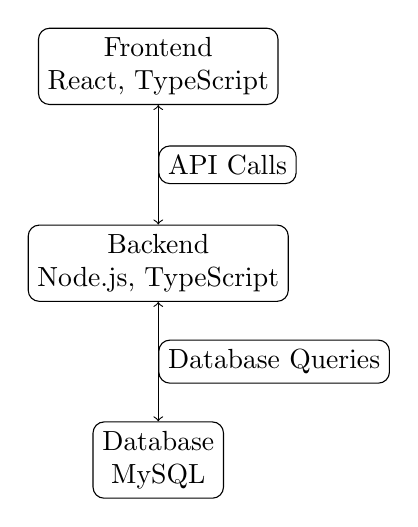
\begin{tikzpicture}[node distance=2.5cm, every node/.style={draw, align=center, rounded corners}]
        \node (frontend) {Frontend \\ React, TypeScript};
        \node (backend) [below of=frontend] {Backend \\ Node.js, TypeScript};
        \node (database) [below of=backend] {Database \\ MySQL};

        \draw[<->] (frontend) -- node[right] {API Calls} (backend);
        \draw[<->] (backend) -- node[right] {Database Queries} (database);
    \end{tikzpicture}
    \caption{Simplified Technology Stack Architecture.}
    \label{fig:tech_stack}
\end{figure}

\subsubsection{Frontend}
The \textbf{\gls{frontend}} is the part of the application users directly interact with. It is responsible for presenting data clearly and intuitively.

\paragraph{React}
React is a \gls{javascript} library designed to simplify the creation of interactive user interfaces by breaking them into reusable components \autocite{react}. We chose React because it allowed us to efficiently build modular, easily maintainable interface components, ensuring consistency and ease of future development. 

\paragraph{Vite}
\gls{vite} is a modern build tool for React that speeds up development by quickly updating changes made to the code \autocite{viteGuide}. It's "Hot Module Replacement" (HMR) feature allow us to instantly view changes during development without refreshing the entire page, speeding up or workflow. 

\paragraph{Typescript}
{\gls{typescript}} enhances {\gls{javascript}} by adding static typing, helping to catch errors early in the developement process. Using Typescripts enures fewer runtime errors, clearer code structure, and overall better quality, significantly benefiting our development efficiency.

\paragraph{MUI}
MUI (Material UI) is a React component library offering ready-made, visually appealing components \autocite{Mui}. We used MUI primarily to speed up frontend development and ensure a consistent visual style across our application. Additionally, MUI simplified creating responsive designs that adapted seamlessly to various screen sizes, improving user experience.

\subsubsection{Backend}
The \textbf{\gls{backend}} handles the application's logic, including data processing, interactions with the database, scheduled tasks, and providing data to the \gls{frontend} via \acrshort{api}s. \gls{backend} technologies were carefully selected to ensure stability and efficient handling of system operations.

\paragraph{Node.js}
Node.js is a runtime environment enabling {\gls{javascript}} code to run outside web browsers, often used for server-side applications \autocite{node}. We chose Node.js for our \gls{backend} because it efficiently handles real-time data and asynchronous operations, critical for our monitoring tasks, such as checking website status regularly.

\paragraph{Axios}
Axios is a \acrshort{http} client that simplifies sending requests between servers and external services. We specifically used \gls{axios} to regularly check the status of each monitored website, collecting key data that users could then present to their clients through the dashboard.

\paragraph{Cron}
\gls{cron} is a scheduling tool enabling tasks to run automatically at set intervals \cite{cron}. We used Cron to schedule website checks, ensuring websites were monitored consistently at defined intervals, and for routine tasks like cleaning old data from the database.

\subsubsection{Database}
The \gls{database} securely stores critical data, including user details, monitored website information, historical status records, incidents, and alerts.

\paragraph{MySQL}
\gls{mysql} is a reliable and widely-used relational database system designed for structured data storage. We chose \gls{mysql} for its robust performance and excellent compatibility with our \gls{backend} technologies. It efficiently handled storing and retrieving large amounts of monitoring data, ensuring quick response times for users accessing the dashboard. See \autoref{fig:mysql_schema} for our database model. The full ER diagram is available in Appendix~\ref{app:ER-Diagram}.

\begin{figure}[H]
    \centering
    \includegraphics[width=1\textwidth]{figures/mysql_scheme.png}
    \caption{Database schema as implemented in MySQL.}
    \label{fig:mysql_schema}
\end{figure}

\subsubsection{Collaboration Technologies}
\label{subsubsec:collab_tech}
To effectively manage teamwork and workflow, we used tools for version control, issue tracking, and collaborative problem-solving. These tools significantly improved our development productivity and quality.

\paragraph{GitHub}
\gls{github} facilitated our collaborative coding by providing a platform for code storage, version control, and code reviews. We used GitHub branches to simultaneously develop new features without interfering with other team members. Each new feature or bug fix was created in its own branch and reviewed thoroughly before merging into our main branch, maintaining code quality. \gls{github-actions} were also used for automated testing and deployment, descibed further in Section \ref{sec:testing_deployment}.

\paragraph{Jira} 
Jira, integrated with our Kanban methodology, provided a clear and structured way to manage tasks. Jira allowed us to create and organize issues derived from application requirements, which we then broke down into actionable tasks. When tasks were actively worked on, corresponding Git branches were created, ensuring task management was tightly integrated with actual coding activities. Additionally, Jira’s assignment feature clearly showed team member's responsibilities, streamlining team collaboration and workload distribution \autocite{Jira}.

\paragraph{AI Tools}
AI tools such as ChatGPT were used throughout the project to assist in solving complex coding issues, debugging, and suggesting improvements. These tools sped up development significantly. All AI-generated suggestions were carefully reviewed and tested before being included in the final codebase, ensuring consistent high code quality.

\subsubsection{End-to-End Testing}
As our application integrated multiple components, {\gls{e2e-testing}} was critical. E2E tests ensure the entire system works correctly from the user’s viewpoint, verifying that interactions between \gls{frontend}, \gls{backend}, and database function seamlessly.

We used {\gls{cypress}}, a widely adopted {\gls{e2e-testing}} tool known for its simplicity and clear reporting. Our tests simulated real user interactions, such as logging in, interacting with dashboard elements, and validating displayed information. Figure~\ref{fig:cypress_test} illustrates an example of an E2E test.

\begin{figure}[H]
    \centering
    \includegraphics[width=0.8\linewidth]{figures/cypress_test.png}
    \caption{Example of Cypress end-to-end test execution}
    \label{fig:cypress_test}
\end{figure}

\subsubsection{Continuous Integration with GitHub Actions}
To continuously ensure code quality and reliability, we used \gls{github-actions} as our continuous integration (CI) tool. We configured two separate automated workflows:

%Forslag til lengre avsnitt:

\begin{itemize}
    \item \textbf{Cypress workflow}: Automatically executed all end-to-end tests, ensuring critical user interactions functioned correctly.
    \item \textbf{Lint and type-check workflow}: Automatically checked for code formatting consistency (Prettier), coding standards adherence (ESLint), and TypeScript correctness.
\end{itemize}

%Istedenfor dette: 

\begin{itemize}
    \item One workflow executed all \texttt{Cypress} end-to-end tests.
    \item The second performed formatting (\gls{prettier}), \gls{eslint}, and TypeScript static type checking.
\end{itemize}

These workflows automatically triggered with each new update (pull request) submitted to the main branch, immediately alerting us to potential issues. Separating the workflows simplified identifying and resolving specific problems, leading to more manageable troubleshooting and clearer workflow processes. Figure~\ref{fig:lint_typecheck_ci} presents an example of the static analysis workflow in action.

\begin{figure}[H]
    \centering
    \includegraphics[width=1\linewidth]{figures/lint_typecheck_ci.png}
    \caption{CI pipeline running \texttt{Prettier}, \texttt{ESLint}, and TypeScript checks via GitHub Actions}
    \label{fig:lint_typecheck_ci}
\end{figure}

\section{Project Planning and Risk Management}
\label{sec:project_planning_risk}
A well-structured planning process was essential for successfully executing this project. This section outlines how we approached project planning, established the project timeline, identified milestones, and managed potential risks throughout development.

Initially, we conducted a comprehensive planning session where the team analyzed the project brief, clarified client requirements, and determined project scope. We also identified key phases, responsibilities, and tasks to achieve clarity on our goals and expectations. Regular team meetings and open communication channels ensured all members were aligned on objectives and progress, facilitating effective collaboration and early detection of potential challenges.

\subsection{Timeline and Milestones}
\label{subsec:timeline_milestones}
Our development process followed a structured timeline clearly defining each phase and milestone. We used a \gls{ganttchart} to visualize our project schedule, providing an overview of important activities such as requirement elicitation, prototype,- and \acrshort{mvp} development, user testing, and documentation (see Figure~\ref{fig:gantt_dev}).

The project officially commenced in week 3 with a thorough requirement elicitation phase lasting from week 3 to week 15. This phase included detailed analysis of the assignment brief, stakeholder interviews, and initial user-needs assessments. Parallel to this, from weeks 5 to 12, we reviewed relevant literature and design theory, informing the system architecture and usability strategies aligned with our \hyperref[subsec:rq1]{\textit{research question}}.

Prototype development was scheduled for weeks 9 and 10, followed by the first user test in weeks 10 and 11. Feedback from this initial testing informed iterative improvements, ensuring the product continuously evolved based on user input. Development of the \acrshort{mvp} took place primarily between weeks 8 and 15, focusing on implementing essential functionalities. The final \acrshort{mvp} evaluation, refinements, and usability improvements took place in weeks 15 and 16. Throughout the project duration, documentation was continuously updated and finalized in weeks 8 to 19.

\begin{figure}[H]
    \centering
    \makebox[\textwidth][c]{\includegraphics[width=1.2\textwidth]{figures/gantt_development.png}}
    \caption{Gantt chart - Project timeline and development phases}
    \label{fig:gantt_dev}
\end{figure}

\subsection{Risk Assessment and Mitigation}
\label{subsec:risk_analysis}
Our risk assessment approach was structured around proactively identifying and managing potential issues to minimize disruptions during development. Risks were assessed based on two main factor: the \textit{likelihood} of occurrence and the potential \textit{impact} if they occurred. This structured evaluation allowed us to allocate resources effectively, and addressing high-severity risks before they could affect the project.

The risk score was determined using the enhanced Sutton matrix (Figure~\ref{fig:risk_matrix}), where the combination of likelihood and impact corresponds to a predefined severity value.

\begin{figure}[H]
    \centering
    \includegraphics[width=0.70\linewidth]{figures/risk_matrix.png}
    \caption{Enhanced risk matrix adapted from Sutton \autocite[Figure 6.2]{Sutton2021}}
    \label{fig:risk_matrix}
\end{figure}

Table \ref{tab:risk_matrix_table} provides an overview of eight significant risks identified, along with their assessed severity and the mitigation strategies applied. This systematic approach helped us respond quickly and efficiently to potential problems, maintaining smooth project progression and avoiding substantial delays.

\begin{table}[H]
    \centering
    \renewcommand{\arraystretch}{1.3}
    \resizebox{\textwidth}{!}{
    \begin{tabular}{|>{\RaggedRight\arraybackslash}p{3.8cm}|l|l|c|>{\RaggedRight\arraybackslash}p{5.5cm}|}
        \hline
        \textbf{Risk} & \textbf{Likelihood} & \textbf{Impact} & \textbf{Score (Sutton)} & \textbf{Mitigation Strategy} \\
        \hline
        R1: Underestimation of development tasks & Likely (4) & Major (4) & 21 &
        Use Kanban board and regular status meetings to reassess progress. Break tasks into smaller units and adjust timeline accordingly. \\
        \hline
        R2: Misalignment of user needs and implemented features & Possible (3) & Critical (5) & 18 &
        Conduct early and repeated user testing with actual stakeholders. Use feedback to update requirements and design decisions. \\
        \hline
        R6: Inadequate testing leads to undetected bugs & Possible (3) & Critical (5) & 18 &
        Integrate automated E2E testing (Cypress) and manual exploratory tests. Apply CI with GitHub Actions for early error detection. \\
        \hline
        R4: Technical unfamiliarity with tools or frameworks & Possible (3) & Major (4) & 16 &
        Allocate time for learning and experimentation early in the project. Use stable technologies and pair programming where necessary. \\
        \hline
        R7: Delays caused by unclear or shifting requirements & Possible (3) & Major (4) & 16 &
        Maintain continuous stakeholder communication. Use agile methods with flexibility to re-prioritize. \\
        \hline
        R8: Frontend-backend integration issues & Possible (3) & Major (4) & 16 &
        Define API interfaces early. Manually test integration points incrementally and regularly. \\
        \hline
        R3: Availability of test users & Possible (3) & Moderate (3) & 15 &
        Coordinate early with Headspin for test scheduling. Conduct on-site sessions and communicate clearly about time expectations. \\
        \hline
        R5: Data loss or versioning errors & Unlikely (2) & Critical (5) & 10 &
        Use GitHub with regular commits and branching. Maintain cloud backups and review pull requests before merges. \\
        \hline
        R9: Team member absence & Unlikely (2) & Major (4) & 9 &
        Maintain clear internal communication and distribute documentation responsibilities across team members. Transparent issue assignment on the Kanban board. \\
        \hline
    \end{tabular}
    }
    \caption{Updated risk assessment with scores based on Sutton’s enhanced risk matrix (Figure~\ref{fig:risk_matrix})}
    \label{tab:risk_matrix_table}
\end{table}

\section{Requirement Elicitation}
\label{sec:req_gathering}
Gathering accurate and comprehensive requirements was essential to developing an effective dashboard application tailored specifically to Headspin AS’s needs. This section outlines our process for eliciting and refining these requirements and explains how they evolved through our incremental development process.

We made an early decision not to elicit requirements related directly to visual design, as Headspin provided us complete freedom in this area. Instead, design decisions were based on principles outlined in \autoref{ch:theory}, supported by direct feedback gathered from user tests.


\subsection{Initial Requirement Analysis and Stakeholder Communication}
\label{subsec:init_req_analysis}
The initial phase of the project involved a thorough analysis of the assignment brief provided by Headspin (Appendix ~\ref{app:headspin-brief}). This review clarified the technical scope and overall objectives of the project and enabled the identification of core expectations. Based on this analysis, an initial set of \textit{\gls{functionalreq}} and \textit{\gls{nonfunctionalreq}} was established, following the structure outlined by Sommerville (\cite[84–91]{sommerville-2011}) (Appendix \ref{app:req_from_brief}).

To validate and expand upon these preliminary requirements, a clarification meeting was held with stakeholders at Headspin. This meeting revealed two primary user groups with differing priorities. Employees engaged in client communication emphasized the need for historical uptime summaries, whereas developers prioritized access to real-time data. The discussion also highlighted the importance of personalization and filtering capabilities within the dashboard. Insights from this meeting led to several adjustments and additions to the requirements, as documented in Appendix \ref{app:req_from_stakeholder}.


\subsection{Prototyping}
\label{subsec:prototyping}
Using the design tool \textit{\gls{figma}}, we created an interactive \gls{prototype} to explore key visualization and navigation aspects. Prototypes, as stated by \textcite[ 423]{sharp-2019}, effectively communicate design concepts and help stakeholders visualize the final product. Prototyping provided a practical way to validate and refine our requirements through conceptual functionality. This means that the prototype was created to only show how the application was intended to function, without spending time actually implementing functionality. This was done to start gathering feedback as early in the project timeline as possible. 

Our prototype supported our incremental development process, by allowing us to gather early feedback in user test 1, as outlined in \autoref{sec:user_testing}. This feedback shaped the requirements that were used to develop the MVP of the application, aligning them closely with user expectations. These requirements are shown in \autoref{ch:results}.

\subsection{Minimum Viable Product}
\label{subsec:mvp}
A \textit{\acrfull{mvp}} is a version of a product developed with just enough features to be usable by  stakeholders. The team developed it using revised requirements after feedback from user test 1. The goal of an MVP is to gather real-world feedback, allowing further enhancements based on practical usage and user insights.

After developing our MVP, we conducted \textit{\hyperref[sec:user_testing]{user test 2}} to gather further insights. This test was an important part of our incremental development process, to identify areas for improvement regarding design and functionality of the application, and to assess overall usability of the system. Based on feedback from user test 2 using the MVP, we categorized our requirements into two lists: one showing completed requirements and another outlining requirements for possible future work. Both lists are provided and explained in detail in Chapter \ref{ch:results}.

\subsection{Requirement prioritization}
\label{subsec:req_prio}
It was important for the team to know what requirements were most important to work on at all times. To accomplish this, all elicited requirements were prioritized during all three stages of requirement elicitation.  all elicited requirements were prioritized according to three main criteria:

\begin{enumerate}
    \item \textbf{Importance to stakeholders} at Headspin.
    \item \textbf{Criticality to core operations}, whether the system’s basic functionality depended on them.
    \item \textbf{Implementation complexity}, considering technical difficulty, required resources, and time needed for completion.
\end{enumerate}

Requirements were then organized into three priority levels:

\begin{enumerate}
    \item \textbf{High-priority:} Essential features for basic usability and core functionality, forming the backbone of the MVP.
    \item \textbf{Medium-priority:} Useful features enhancing user experience but not critical for basic operation.
    \item \textbf{Low-priority:} Optional improvements, to be considered if time and resources permitted after addressing higher priorities.
\end{enumerate}

This prioritization strategy allowed transparent decision-making and supported our agile, iterative development approach. It also facilitated the flexibility needed to re-prioritize requirements based on ongoing feedback from user testing.

\section{User Testing Methodology}
\label{sec:user_testing}
User testing was an essential part of the iterative development process, helping us continuously improve both the functionality and usability of our dashboard application. To properly evaluate our design decisions and measure user experience, we conducted two separate user tests at different stages of development:

\begin{itemize}
    \item \textbf{User Test 1} evaluated an interactive \textit{\hyperref[fig:prototype_dashboard]{prototype}}, designed to validate initial ideas before major development began.
    \item[] 
    \item \textbf{User Test 2} evaluated a working \textit{\acrshort{MVP}}, allowing us to measure actual usability and user experience. 
\end{itemize}

In the following sections, we explain in detail how we chose participants, how each test was structured, and how we collected and analyzed data. Results from both tests are presented in chapter~\ref{ch:results}.

\subsection{Participant Selection}
\label{subsec:participant_selection}
Participants for both tests were employees at Headspin AS, recruited internally from roles related to web development, design, and project management. By selecting people from various backgrounds within the company, we ensured a balanced mix of technical and design perspectives. To achieve better consistency and allow direct comparison between both user tests, the same participants were involved in both testing sessions.

All participants provided informed consent, and the tests were conducted at Headspin’s office in Trondheim. This created a familiar environment for the participants, helping them feel comfortable and reducing potential bias caused by external factors.

\subsection{User Test 1: Prototype Evaluation}
\label{subsec:user_test_1}
The first user test aimed to confirm our initial design decisions early in the project, using a clickable prototype built in \gls{figma}. This test allowed us to quickly identify any issues or misunderstandings regarding the layout, design, and expected functionality before we began more complex development work.
Each session followed the same structured procedure, ensuring consistency and comparability:

\begin{itemize}
    \item \textbf{Briefing:}
    Each participant was welcomed and introduced to the purpose of the test. They were assured that we were testing the prototype, not them, and encouraged to speak openly about their thoughts. We explained the \textit{\gls{thinkaloudprotocol}}, asking participants to say out loud what they were thinking during the tasks.
    \item[] 
    \item \textbf{Task Execution:}
    Participants were asked to complete five predefined tasks designed to thoroughly test key parts of the prototype, such as navigation and interaction with specific features. These tasks were realistic scenarios similar to what the users would encounter during daily use (see Appendix~\ref{app:prototype_testplan} for detailed tasks). One team member led each session, while other team members took notes and recorded observations.
    \item[] 
    \item \textbf{Post-Test Interview:}
    After the task session, participants were interviewed using a semi-structured approach. We asked participants predefined questions as well as spontaneous follow-up questions based on their comments and interactions during testing. This helped identify deeper issues related to usability or design that might not have been apparent during the tasks alone.
\end{itemize}

\subsection{User Test 2: MVP evaluation}
\label{subsec:user_test_2}
The second user test evaluated the developed \textit{\acrshort{mvp}}, a fully functioning but simplified version of our dashboard application. The goal was to measure how well our design and functionality improvements, made after feedback from user test 1, worked in practice.
The test followed the same general format as the prototype test (briefing, think-aloud, tasks, and interviews), but had some important differences. 

Participants interacted with a fully functioning system, rather than a prototype. This allowed us to test realistic interactions, system responsiveness, and actual implementation of features. The tasks used in this test covered additional features and functionalities that were not available in the initial prototype, such as user login, managing website data, and changing settings. This reflected the enhanced capabilities of our \acrshort{mvp}, and gave a more complete picture of overall usability (see Appendix~\ref{app:mvp_testplan}).

After finishing all tasks, participants completed a standardized questionnaire (System Usability Scale, or \textit{\acrshort{sus})}. This step was completed immediately after testing, before any discussion, to ensure that their responses were based only on their direct experience, and not influenced by subsequent discussions.

\subsection{\acrlong{sus}}
\label{subsec:sus}
To quantitatively evaluate how users perceived the usability of our MVP, we used the \acrfull{sus}. \acrshort{sus} is a widely recognized questionnaire that contains ten simple statements. Participants rated each statement from 1 ("Strongly disagree") to 5 ("Strongly agree") on a standardized five-point scale called a \gls{likertscale} \autocite{MeasuringSUS2011}.

After users completed the questionnaire, we calculated a \acrshort{sus} score between 0 and 100. It’s important to note that this score is not a simple percentage, but rather a standardized usability measure. Typically, scores above 68 indicate above-average usability, and scores of 85 or higher represent excellent usability.

The exact method for calculating SUS scores and the complete SUS questionnaire used in our second user test are provided in Appendix~\ref{app:sus_calculation}. Results and detailed analysis of SUS scores are presented in chapter~\ref{ch:results}, Section~\ref{subsec:quant_sus}, where they are discussed in combination with qualitative user feedback.

\subsection{Data Collection and Analysis}
Throughout both user tests, we carefully recorded data using three main methods:

\begin{itemize}
    \item \textbf{Direct observation:}
    Observations during task execution helped us understand user's interactions and immediate reactions to the system.
    \item \textbf{Detailed note-taking:}
    Team members took structured notes about participant actions, challenges, and verbal comments.
    \item \textbf{Post-test interviews:}
    Interviews allowed us to discuss the participant’s experiences more deeply and identify usability problems that might have been missed during direct observation. 
\end{itemize}

After each round of testing, our team gathered to analyze the collected data. We identified common patterns and recurring issues, using these insights to refine both design and functionality. Feedback from both tests informed our iterative improvement process and helped us update our project requirements accordingly (see Section~\ref{sec:req_gathering}).

In the second test, the SUS questionnaire provided additional numerical data that complemented our qualitative observations, giving us a clearer overall assessment of system usability.


\subsection*{Summary of Requirement Elicitation and User Testing}

To summarize how our requirement elicitation and user testing processes were interconnected throughout the project timeline, we created an overview that visualizes the iterative flow between key development activities. As the timeline illustrates, each phase, from the initial analysis to the final application, was followed by corresponding user tests and requirement elicitation, and prioritization cycles. These cycles allowed us to continuously refine and adjust requirements based on real user input. 

\autoref{fig:iterative_methodology_timeline} outlines this progression and highlights how requirement elicitation and user testing informed each other throughout the development process.

\begin{figure}[H]
    \centering
    \resizebox{0.75\textwidth}{!}{%
        \begin{tikzpicture}[
            node distance=1.5cm and 2.2cm,
            stage/.style={rectangle, rounded corners, draw=black, fill=gray!10, text width=5cm, align=center, font=\small},
            activity/.style={ellipse, draw=black, fill=blue!5, text width=3.2cm, align=center, font=\small},
            arrow/.style={-Latex, thick},
            flow/.style={->, very thin, dashed, gray},
            every node/.append style={inner sep=6pt}
        ]

        \node (analysis) [stage] {Initial Requirement Analysis\\\& Stakeholder Meeting};
        \node (prio1) [activity, below=of analysis] {Requirement\\Prioritization};
        \node (proto) [stage, below=of prio1] {Prototyping};
        \node (prio2) [activity, below=of proto] {Requirement\\Prioritization};
        \node (mvp) [stage, below=of prio2] {MVP Development};
        \node (prio3) [activity, below=of mvp] {Requirement\\Prioritization};
        \node (final) [stage, below=of prio3] {Final Application\\(Post-MVP Improvements)};

        \node (test1) [activity, right=of proto] {User Test 1};
        \node (test2) [activity, right=of mvp] {User Test 2};

        \draw[arrow] (analysis) -- (prio1);
        \draw[arrow] (prio1) -- (proto);
        \draw[arrow] (proto) -- (prio2);
        \draw[arrow] (prio2) -- (mvp);
        \draw[arrow] (mvp) -- (prio3);
        \draw[arrow] (prio3) -- (final);

        \draw[arrow] (proto.east) -- (test1.west);
        \draw[arrow] (mvp.east) -- (test2.west);

        \draw[arrow] (test1.south) -- ++(0,-0.5) -| (prio2.east);
        \draw[arrow] (test2.south) -- ++(0,-0.5) -| (prio3.east);

        \draw[flow] (prio1.south) -- ++(0,-0.3) -| (prio2.north);
        \draw[flow] (prio2.south) -- ++(0,-0.3) -| (prio3.north);

        \end{tikzpicture}%
    }
    \caption{Timeline showing iterative refinement through requirement prioritization and user testing}
    \label{fig:iterative_methodology_timeline}
\end{figure}



\subsection{Validity and Reliability}
Assessing validity and reliability ensures the quality and credibility of our results. Reliability means that our methods were consistent enough to give similar results if repeated. Validity ensures that we collected data relevant to our research question \autocite[240-241]{grønmo}.

\subsubsection{Validity}
\label{subsubsec:validity}
To ensure our study had high validity, we chose methods specifically suited to our research goals. Qualitative methods (interviews, observations) helped us gather detailed user feedback, while quantitative methods (SUS questionnaire) provided clear usability metrics. Combining these methods allowed us to cross-check results, increasing our confidence in their accuracy.

We carefully selected test participants who represented actual users at Headspin AS. By involving these relevant stakeholders, we made sure our results reflected real-world conditions (ecological validity). Tasks were realistic and mirrored everyday situations, enhancing both internal validity (ensuring user feedback was clearly linked to our design decisions) and external validity (ensuring results apply broadly to practical use).

\subsubsection{Reliability}
\label{subsubsec:reliability}
To achieve reliability, we ensured consistency in all user tests. Participants received identical tasks and instructions, using standardized scripts. We also employed the same structured SUS questionnaire each time, providing repeatable, comparable usability measures.

However, factors like individual differences between participants (experience, skills, personal preferences) inevitably introduced slight variations in responses. Additionally, interpreting qualitative feedback could involve some subjective judgment by our team. To manage this, we carefully documented our procedures and interpretations clearly, so anyone repeating our study could replicate our approach and assess reliability effectively.

Through structured testing methods, detailed documentation, and careful participant selection, we sought to maximize reliability while openly acknowledging its natural limitations.